\documentclass[border=4pt]{standalone}

\usepackage[T1]{fontenc}
\usepackage[utf8]{inputenc}
\usepackage{amsmath}
\usepackage{xcolor}
\usepackage{tikz}

\begin{document}

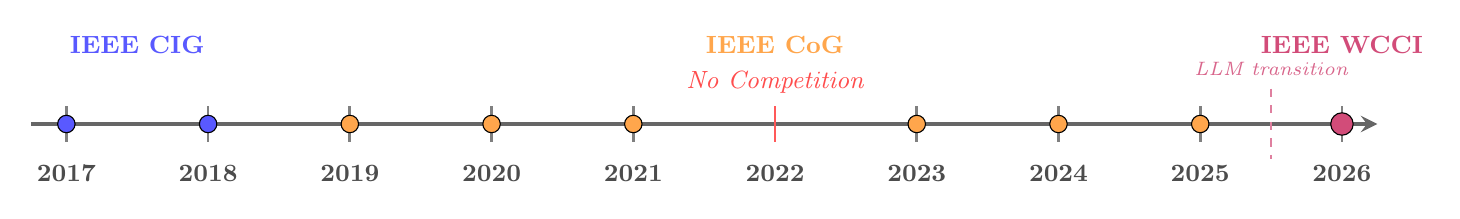
\begin{tikzpicture}[scale=0.9]
% Timeline axis
\draw[->, >=stealth, line width=1.6pt, black!60] (-0.5,0) -- (18.5,0);

% Year ticks
\foreach \x/\year in {0/2017,2/2018,4/2019,6/2020,8/2021,10/2022,12/2023,14/2024,16/2025,18/2026} {
    \draw[line width=1pt, black!50] (\x,0.25) -- (\x,-0.25);
    \node[font=\small\bfseries, black!70] at (\x,-0.7) {\year};
}

% 2017–2018: IEEE CIG
\filldraw[fill=blue!65] (0,0) circle (3.5pt);
\filldraw[fill=blue!65] (2,0) circle (3.5pt);
\node[anchor=south, font=\small\bfseries, align=center, text=blue!65] at (1,0.85) {IEEE CIG};

% 2019–2021 and 2023–2025: IEEE CoG
\foreach \x in {4,6,8,12,14,16} {
    \filldraw[fill=orange!70] (\x,0) circle (3.5pt);
}
\node[anchor=south, font=\small\bfseries, align=center, text=orange!70] at (10,0.85) {IEEE CoG};

% 2022: No competition
\draw[line width=1pt, red!65] (10,0.25) -- (10,-0.25);
\node[font=\small\itshape, text=red!70, anchor=south] at (10,0.3) {No Competition};

% Subtle paradigm shift marker
\draw[dashed, line width=0.8pt, purple!50] (17, 0.5) -- (17, -0.5);
\node[font=\scriptsize\itshape, text=purple!60, anchor=south, fill=white, inner sep=2pt] at (17, 0.6) {LLM transition};

% 2026: IEEE WCCI
\filldraw[fill=purple!70] (18,0) circle (4.5pt);
\node[anchor=south, font=\small\bfseries, align=center, text=purple!70] at (18,0.85) {IEEE WCCI};
\end{tikzpicture}

\end{document}
